\documentclass[12pt]{beamer}
\usepackage[utf8]{inputenc}
\usepackage[T1]{fontenc}
\usepackage{graphicx}
\usepackage{gensymb}
\usepackage{lmodern}
\usetheme{PaloAlto}
\begin{document}
	\author{Leonardo Testolin - VR436823}
	\title{Diverse soluzioni e sfide per gli schermi AMOLED e OLED}
	\subtitle{Relazione Fisica dei Dispositivi Integrati}
	%\logo{}
	%\institute{}
	%\date{}
	%\subject{}
	\setbeamercovered{transparent}
	%\setbeamertemplate{navigation symbols}{}
	\begin{frame}[plain]
		\maketitle
	\end{frame}
	
	\begin{frame}
		\frametitle{Introduzione: alcuni concetti base}
		\begin{figure}[h]
			\centering
			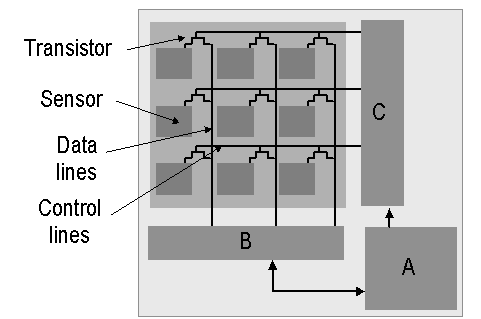
\includegraphics[width=0.9\textwidth]{IMMAGINI/arraydiag}
			\caption{Transistor TFT}
			\label{TFT}
		\end{figure}
	\end{frame}
	\begin{frame}
		\frametitle{Introduzione: alcuni concetti base}
		\begin{figure}
			\centering
			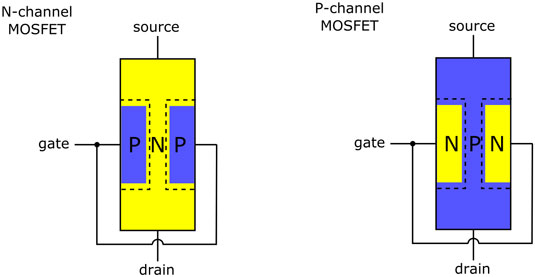
\includegraphics[width=1\linewidth]{IMMAGINI/FET_DET}
			\caption{Transistor FET}
			\label{fig:fetdet}
		\end{figure}
	\end{frame}
	\begin{frame}
		\frametitle{Introduzione: alcuni concetti base}
		\begin{figure}
			\centering
			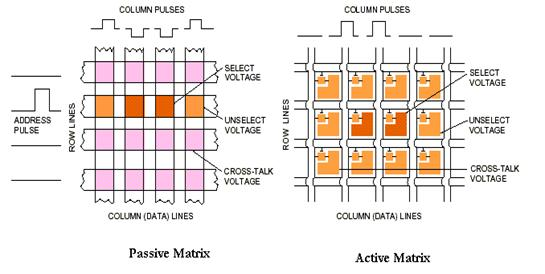
\includegraphics[width=1\linewidth]{IMMAGINI/matrix_passive}
			\caption{ Passive Matrix and Active Matrix}
			\label{fig:matrixpassive}
		\end{figure}
	\end{frame}
	\begin{frame}
		\frametitle{Introduzione: alcuni concetti base}
		\begin{figure}
			\centering
			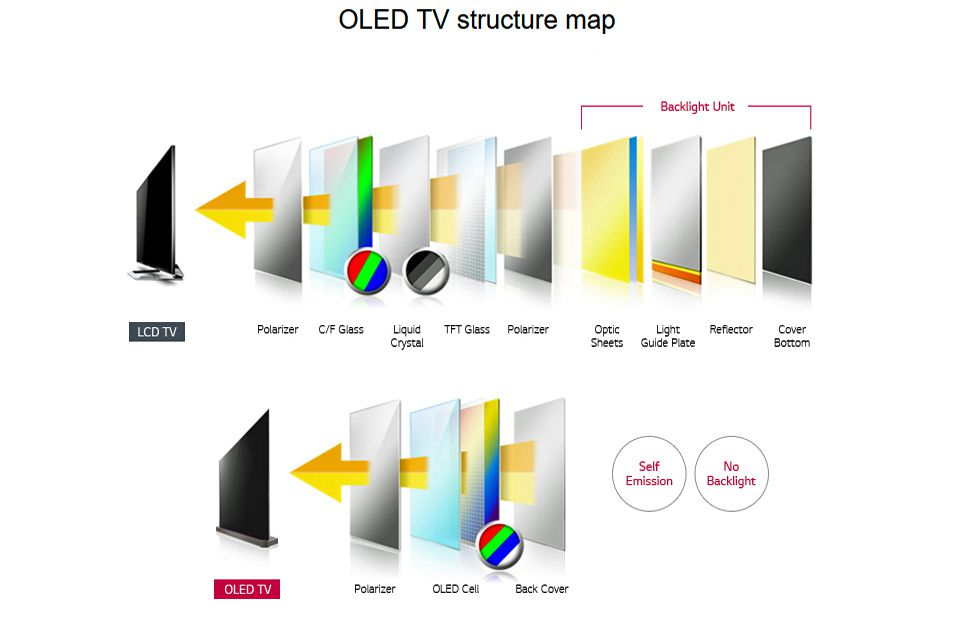
\includegraphics[width=1\linewidth]{IMMAGINI/OLED_vs_LCD}
			\caption{OLED vs LCD}
			\label{fig:oledvslcd}
		\end{figure}	
	\end{frame}
	\begin{frame}
		\frametitle{Introduzione: alcuni concetti base}
		\begin{figure}
			\centering
			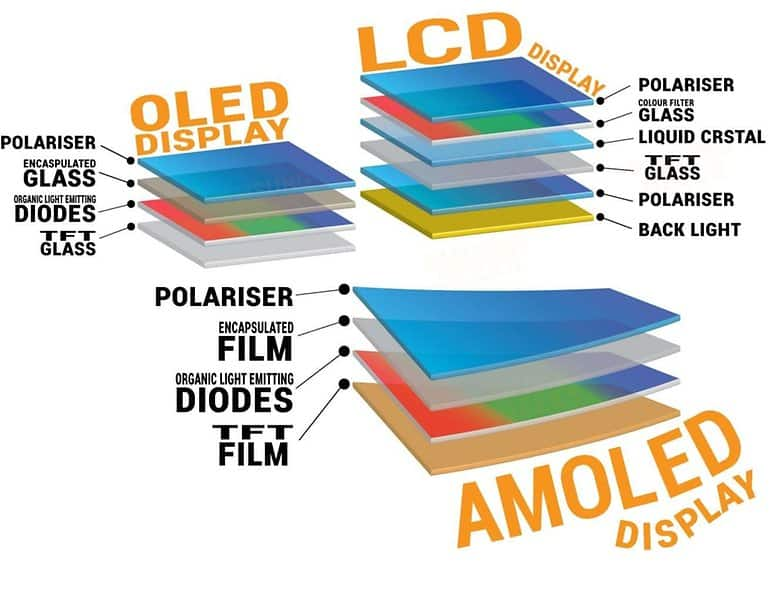
\includegraphics[width=0.8\linewidth]{IMMAGINI/AMOLED_VS_LCD}
			\caption{AMOLED vs LCD}
			\label{fig:amoledvslcd}
		\end{figure}	
	\end{frame}
	\begin{frame}
		\frametitle{Introduzione: alcuni concetti base}
		\begin{figure}
			\centering
			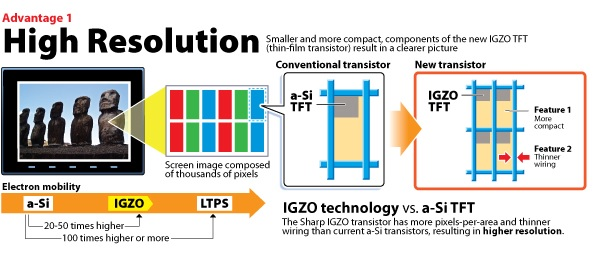
\includegraphics[width=1\linewidth]{IMMAGINI/IGZO-vs-aSi-1}
			\caption{IGZO vs a-Si}
			\label{fig:igzo-vs-asi-1}
		\end{figure}
	\end{frame}
	\begin{frame}
		\frametitle{Introduzione: alcuni concetti base}
		\begin{figure}
			\centering
			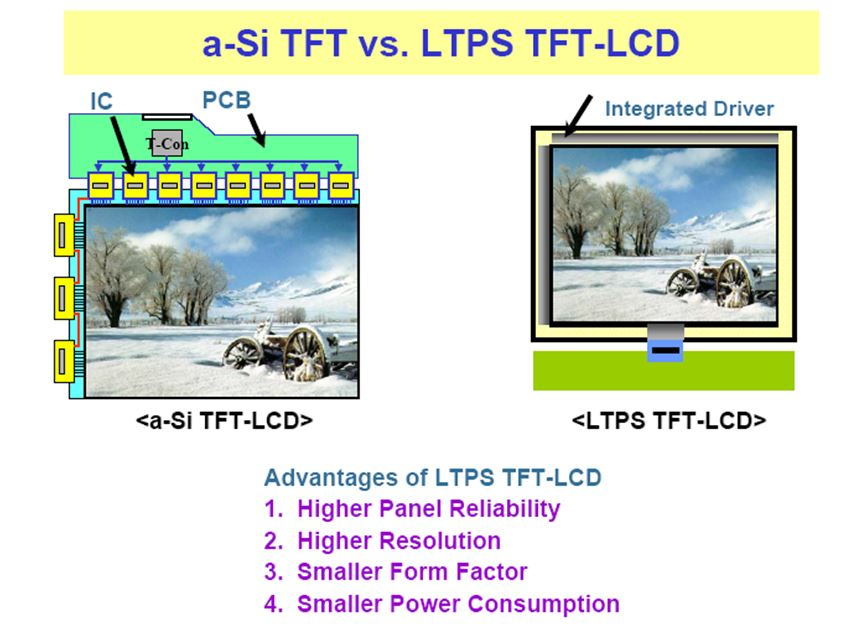
\includegraphics[width=1\linewidth]{IMMAGINI/ltps-(technology)}
			\caption{LTPS-technology}
			\label{fig:ltps-technology}
		\end{figure}
	\end{frame}
	\begin{frame}
		\frametitle{24-INCH WIDE UXGA TFT-LCD per applicazioni HDTV}
		\begin{itemize}
			\item Sorgono molti problemi nella creazione di schermi di grandi dimensioni
			\pause
			\item Molti approcci sono stati adottati per cercare di superare l’insufficienza della ricarica del pannello,
			cercando di usare tecniche guidate, cercando di manipolare il tempo di ricarica
			\pause
			\item Quando pixel e dimensione dello schermo aumentano, il consumo energetico che deve essere fornito ai pixel diventa un problema molto critico
		\end{itemize}
	\end{frame}
	\begin{frame}
		\frametitle{24-INCH WIDE UXGA TFT-LCD per applicazioni HDTV}
		\begin{itemize}
			\item I problemi maggiori sono legati anche a problemi di ritardo e la distorsione data dall'alta resistenza e capacità parassitaria
		\end{itemize}
	\end{frame}
	\begin{frame}
		\frametitle{24-INCH WIDE UXGA TFT-LCD per applicazioni HDTV}
		\begin{figure}
			\centering
			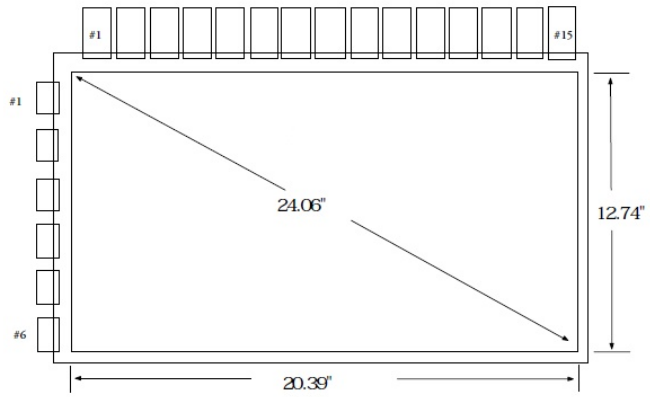
\includegraphics[width=1\linewidth]{IMMAGINI/schermoLCD}
			\caption{Schermo LCD}
			\label{fig:schermolcd}
		\end{figure}
	\end{frame}
	\begin{frame}
		\frametitle{24-INCH WIDE UXGA TFT-LCD per applicazioni HDTV}
		\begin{itemize}
			\item Dall’analisi di alcuni risultati, si è potuto notare che i ritardi sulle gate line  causano insufficienza di carica nei pixel causando lo sfarfallio dello schermo, mentre i ritardi sulle data line causano insufficienza di carica nei pixel relativi al cross-talk verticale
		\end{itemize}
	\end{frame}
	\begin{frame}
	\frametitle{24-INCH WIDE UXGA TFT-LCD per applicazioni HDTV:  Metodi}
		\begin{itemize}
			\item Se ci sono questi problemi è possibile implementare lo split delle data line
			\pause
			\item Si riduce così il clock e il data rate abbastanza
			da usare un device con frequenze molto più basse
			\pause
			\item 4 differenti bus dati sono richiesti per poter gestire questi 4 blocchi dati differenti
		\end{itemize}
	\end{frame}
	\begin{frame}
		\frametitle{24-INCH WIDE UXGA TFT-LCD per applicazioni HDTV:  Metodi}
		\begin{figure}
			\centering
			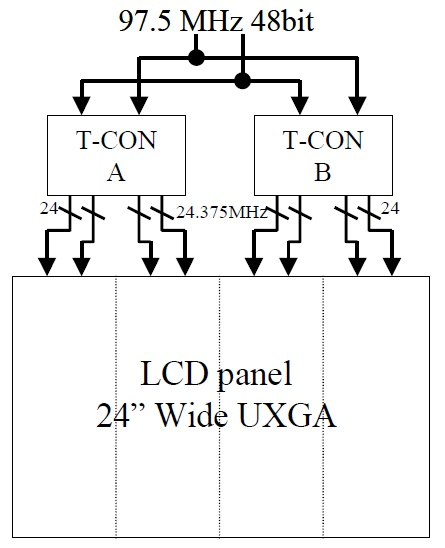
\includegraphics[width=0.5\linewidth]{FISICA/T-CON}
			\caption{T-CON}
			\label{fig:t-con}
		\end{figure}
	\end{frame}
	\begin{frame}
		\frametitle{24-INCH WIDE UXGA TFT-LCD: Configurazione di sistema}
		Un sistema totale usato per un display WUXGA consiste di 3 parti:
		\begin{itemize}
			\item Scheda video
			\item Interfaccia IC
			\item Modulo TFT-LCD di 24-inch
		\end{itemize}
	\end{frame}
	\begin{frame}
		\frametitle{24-INCH WIDE UXGA TFT-LCD: Configurazione di sistema}
		\begin{figure}
			\centering
			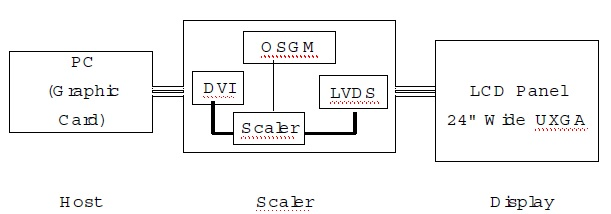
\includegraphics[width=1\linewidth]{FISICA/sistema_di_conf}
			\caption{Configurazione di sistema}
			\label{fig:sistemadiconf}
		\end{figure}
	\end{frame}
	\begin{frame}
		\frametitle{24-INCH WIDE UXGA TFT-LCD: angolo di visione}
		\begin{itemize}
			\item Per migliorare la visione d’angolo dello schermo è stato sviluppato un nuovo
			modello VA (vertical alignment) ridenominato PVA (patterned
			vertical alignment), che utilizza dei campi della frontiera che sono guidati rispettivamente con il modello VA
			\pause
			\item Cosi facendo dopo alcuni test si sono potuti ottimizzare le prestazioni delle celle del display 
		\end{itemize}
	\end{frame}
	\begin{frame}
		\frametitle{Pixel AMOLED basati su circuiti in poly-Si TFTs: introduzione}
		\begin{itemize}
			\item In particolare si fa una comparazione tra accuratezza, velocità di guida, consumo
			energetico e area occupata
		\end{itemize}
	\end{frame}
	\begin{frame}
		\frametitle{Pixel AMOLED basati su circuiti in poly-Si TFTs: introduzione}
		\begin{itemize}
			\item Organic ligth-emitting diode (OLED) sono display che sono efficienti dal punto di vista del consumo energetico,vivido e ideale per applicazioni portatili 
			\pause
			\item Sono costituiti da materiali a basso costo e vengono utlizzati meno processi di produzione per la loro creazione rispetto agli LCDs
		\end{itemize}
	\end{frame}
	\begin{frame}
		\frametitle{Pixel AMOLED basati su circuiti in poly-Si TFTs: introduzione}
		\begin{figure}
			\centering
			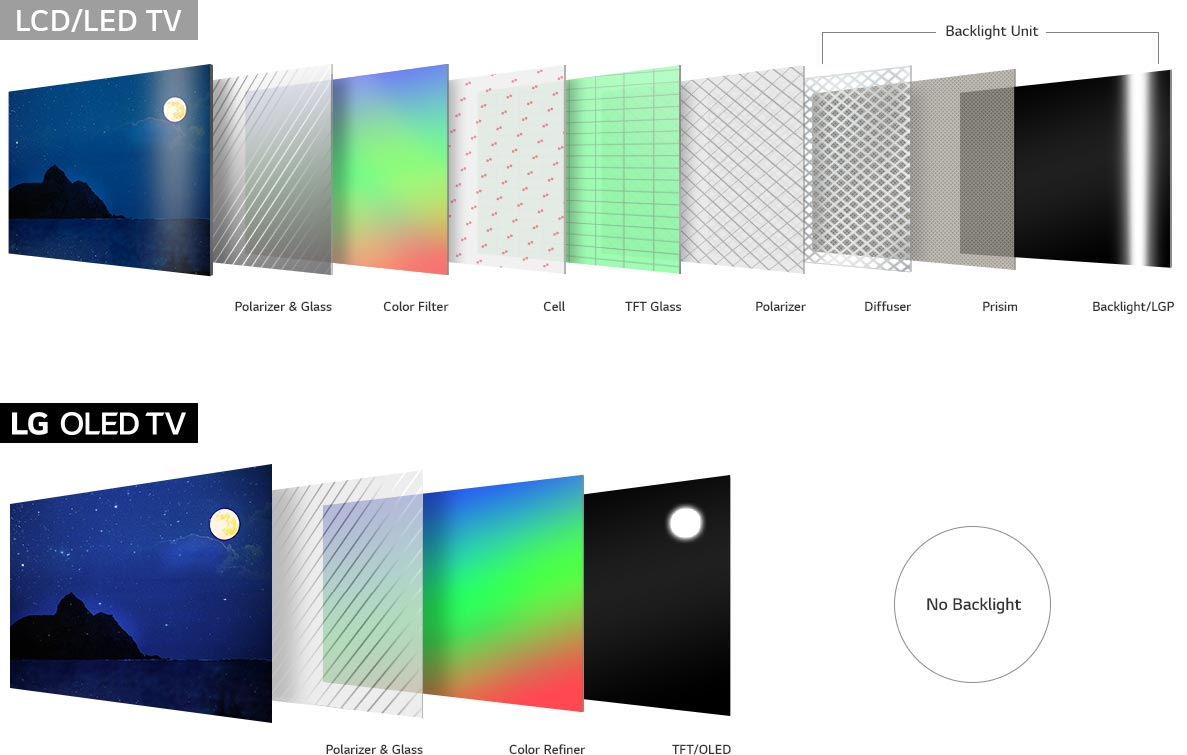
\includegraphics[width=1\linewidth]{IMMAGINI/oled}
			\caption{OLED}
			\label{fig:oled}
		\end{figure}
	\end{frame}
	\begin{frame}
		\frametitle{Pixel AMOLED basati su circuiti in poly-Si TFTs: introduzione}
		\begin{itemize}
			\item L’OLED è un device guidato da corrente dove il livello di luminosità è determinato dal livello di corrente che lo attraversa
		\end{itemize}
	\end{frame}
	\begin{frame}
		\frametitle{Pixel AMOLED basati su circuiti in poly-Si TFTs: introduzione}
		\begin{itemize}
			\item Per queste ragioni gli OLED appaiono i migliori candidati per le diverse applicazioni mobili
			\pause
			\item Questa corrente può essere fornita da una matrice passiva OLED (PMOLED) oppure da una matrice attiva (AMOLED)
		\end{itemize}
	\end{frame}
	\begin{frame}
		\frametitle{Pixel AMOLED basati su circuiti in poly-Si TFTs: introduzione}
		\begin{itemize}
			\item La soluzione proposta prevede un approccio in cui si tende ad utilizzare la matrice passiva, in particolare, quando la dimensione dello schermo va aumentando
			\pause
			\item La matrice passiva richiede un picco elevato di corrente per poter funzionare, ma questo, permette di ottenere alta luminosità
			\pause
			\item Un consumo elevato di energia ha dimostrato effetti di maggior affidabilità da parte degli schermi OLED
		\end{itemize}
	\end{frame}
	\begin{frame}
		\frametitle{Pixel AMOLED basati su circuiti in poly-Si TFTs: Circuiti driver per gli schermi OLED}
		I circuiti OLED possono essere divisi in due classi:
		\begin{itemize}
			\item Circuiti sul voltaggio
			\pause
			\item Circuiti sulla corrente
		\end{itemize}
	\end{frame}
	\begin{frame}
		\frametitle{Pixel AMOLED basati su circuiti in poly-Si TFTs: Voltage-programming driver circuits}
		\begin{itemize}
			\item Il più semplice circuito chiamato 2-TFT, può essere creato tramite due TFT (T1 e T2)
			\pause
			\begin{figure}
				\centering
				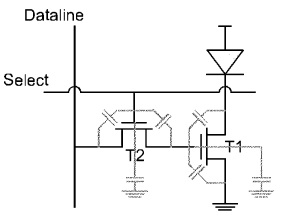
\includegraphics[width=0.7\linewidth]{FISICA/tft_oled_driver}
				\caption{TFT OLED driver}
				\label{fig:tftoleddriver}
			\end{figure}
		\end{itemize}
	\end{frame}
	\begin{frame}
		\frametitle{Pixel AMOLED basati su circuiti in poly-Si TFTs: Voltage-programming driver circuits}
		\textcolor{red}{Problemi:}
		\begin{itemize}
			\item Pesante drenaggio di corrente dovuto alla threshold del TFT
			\item Variazione di mobilità delle cariche
		\end{itemize}
		\pause
		\textcolor{green}{Soluzione:}
		\pause
		\begin{itemize}
			\item Per poter superare questo inconveniente deve essere introdotto un circuito che si auto-compensa, è semplice da realizzare, ma ha bisogno di più componenti
		\end{itemize}
	\end{frame}
	\begin{frame}
		\frametitle{Pixel AMOLED basati su circuiti in poly-Si TFTs: Voltage-programming driver circuits}
		\begin{itemize}
			\item Introducendo questa miglioria, il circuito risultante sarà denominato 4-TFT
		\end{itemize}
		\pause
		\begin{figure}
			\centering
			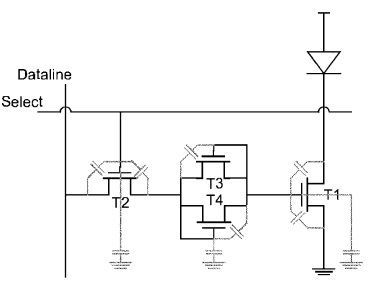
\includegraphics[width=0.7\linewidth]{FISICA/tft_oled_maggiore}
			\caption{TFT OLED major}
			\label{fig:tftoledmaggiore}
		\end{figure}
	\end{frame}
	\begin{frame}
		\frametitle{Pixel AMOLED basati su circuiti in poly-Si TFTs: Current-programming driver circuits}
		Possiamo settare in maniera precisa la corrente che viene data allo schermo OLED con un approccio basato sulla programmazione di corrente
	\end{frame}
	\begin{frame}
		\frametitle{Pixel AMOLED basati su circuiti in poly-Si TFTs: Current-programming driver circuits}
		\begin{figure}
			\centering
			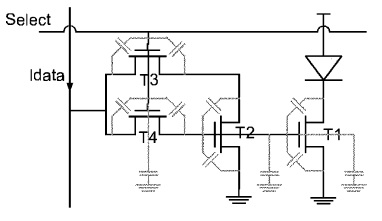
\includegraphics[width=1\linewidth]{FISICA/current_mirror}
			\caption{Current Mirror}
			\label{fig:currentmirror}
		\end{figure}
	\end{frame}
	\begin{frame}
		\frametitle{Pixel AMOLED basati su circuiti in poly-Si TFTs: Current-programming driver circuits}
		Una variante migliore rispetto alla precedente, introduce una circuito driver con memoria. Questo permetterà di ottenere migliori prestazioni in quanto è possibile tenere "in memoria" un certo voltaggio
	\end{frame}
	\begin{frame}
		\frametitle{Pixel AMOLED basati su circuiti in poly-Si TFTs: Current-programming driver circuits}
		\begin{figure}
			\centering
			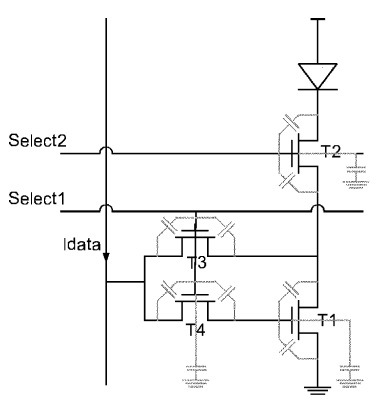
\includegraphics[width=0.6\linewidth]{FISICA/one_tras_current}
			\caption{One-transistor current memory driver circuit}
			\label{fig:onetrascurrent}
		\end{figure}
	\end{frame}
	\begin{frame}
		\frametitle{Pixel AMOLED basati su circuiti in poly-Si TFTs: Velcocità di guida}
		\begin{itemize}
			\item Per calcolare il frame rate dei pixel	si utilizza una formula che considera il numero di righe per matrice, il tempo di ricarica dei capacitori, il tempo di ricarica del capacitore TFT e il tempo di carica e scarica delle righe della matrice
		\end{itemize}
	\end{frame}
	\begin{frame}
		\frametitle{Pixel AMOLED basati su circuiti in poly-Si TFTs: Conclusioni}
		\begin{itemize}
			\item Tra le differenti topologie, la migliore è la 4-TFT con la quale la velocità è 10 volte più alta rispetto alla
			topologia basate su corrente e con un risparmio del 30\% più alto. Però, se il 10\%
			della variazione sul drenaggio della corrente è dovuto alla variazione di mobilità,
			questo non può essere accettato e quindi si passa ad una topologia basata su
			corrente
		\end{itemize}
	\end{frame}
	\begin{frame}
		\frametitle{Display AMOLED pieghevoli: introduzione}
		\begin{itemize}
			\item La fisicità del display risulta essere molto importante in termini di portabilità e design
		\end{itemize}
	\end{frame}
	\begin{frame}
		\frametitle{Display AMOLED pieghevoli: introduzione}
		\begin{itemize}
			\item Ci sono alcuni punti chiave da dover tenere in considerazione quando si parla di display OLED pieghevoli ed è la rottura del display dovuta alla curvatura
			\pause
			\item Di solito,un display OLED include un sottostrato di plastica piuttosto che un sottostrato di vetro
			\pause
			\item La plastica trasmette condensa/umidità; quindi, dei film passivi sono richiesti per poter reagire con l’umidità e la degradazione
		\end{itemize}
	\end{frame}
	\begin{frame}
		\frametitle{Display AMOLED pieghevoli: introduzione}
		\textcolor{green}{Soluzione:}
		\begin{itemize}
			\item Per ridurre, invece, WVRT in maniera sufficiente, un film inorganico deve essere inserto ed essere sufficientemente sottile
			\pause
			\item Il substrato di plastica dell’OLED non può resistere ad alte temperature. Infatti, un film inorganico deve essere
			formato a basse temperature, creando così il film con una bassa densità in relazione alla temperatura
			\pause
			\item Il film deve essere formato in maniera ordinata, eliminando le possibili condense che potrebbero risultare
		\end{itemize}
	\end{frame}
	\begin{frame}
		\frametitle{Display AMOLED pieghevoli: introduzione}
		\textcolor{red}{Alcuni problemi:}
		\begin{itemize}
			\item I film essendo cosi fini, ne compromettono la funzionalità
			\pause
		\end{itemize}
		\textcolor{green}{Soluzione:}
		\begin{itemize}
			\item Si è fabbricato un display AMOLED flessibile usando un \textbf{trasferimento di tecnologia} che implementa la separazione inorganica dei vari livelli
		\end{itemize}
	\end{frame}
	\begin{frame}
		\frametitle{Display AMOLED pieghevoli: CAAC-OS}
		\begin{itemize}
			\item Si è sviluppato un c-axis-aligned-crystal oxide semiconduttore (CAAC-OS) chiamato anche c-axis-aligned-nano-crystal oxide semicondittore (CANC-OS), utilizzato in questo caso per creare il display FET
		\end{itemize}
	\end{frame}
	\begin{frame}
		\frametitle{Display AMOLED pieghevoli: IGZO}
		\begin{itemize}
			\item Possiamo identificare come OS (Ossido semiconduttore) l'IGZO (Indio, Gallio, Zinco)
			\pause
			\item La formazione del CAAC-IGZO come un film sottile su uno strato di vetro è rihiesta la 'ricottura' a meno di 500 \degree C
		\end{itemize}
	\end{frame}
	\begin{frame}
		\frametitle{Display AMOLED pieghevoli: IGZO}
		\begin{itemize}
			\item Lo step successivo è quello di formare uno strato che va ad usare CAAC-IGZO per una livello attivo e cercare di fornire maggiore affidabilità
			\pause
			\item Per il pannello posteriore è stato utilizzato LTPS ovvero il polisilicone a basse temperature
			\pause
			\item \textcolor{red}{LTPS ha alcuni problemi}
		\end{itemize}
	\end{frame}
	\begin{frame}
		\frametitle{Display AMOLED pieghevoli: LTPS problemi}
		\begin{itemize}
			\item I display consumano una grande quantita di corrente dovuta ai livello alti di funzionamento della corrente
			\pause
			\item La fabbricazione richiede molti step, il costo molto elevato e un'equipaggiamento di manifattura non da poco (irradiazione laser)
		\end{itemize}
	\end{frame}
	\begin{frame}
		\frametitle{Display AMOLED pieghevoli: CAAC-OS vantaggi}
		\begin{itemize}
			\item Consumo di energia per la visualizzazione dell'immagine molto basso dovuto a livello di funzionamento della corrente molto basso
			\pause
			\item Non sono richieste presenza di laser a differenza di LTPS
		\end{itemize}
	\end{frame}
	\begin{frame}
		\frametitle{Display AMOLED pieghevoli: Cristallizzazione}
		\begin{figure}
			\centering
			\includegraphics[width=1\linewidth]{"IMMAGINI/Cristalizzazione CAAS"}
			\caption{Crystals}
			\label{fig:cristalizzazione-caas}
		\end{figure}
	\end{frame}
	\begin{frame}
		\frametitle{Display AMOLED pieghevoli: Cristallizzazione}
		\begin{figure}
			\centering
			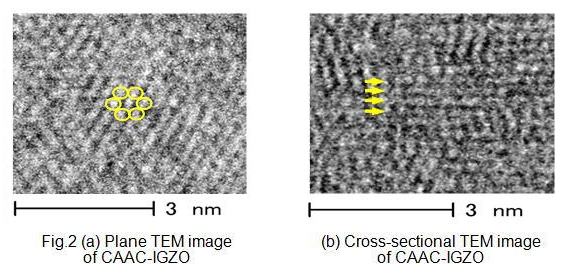
\includegraphics[width=1\linewidth]{IMMAGINI/immagine_cristalizzazione}
			\caption{Crystals}
			\label{fig:immaginecristalizzazione}
		\end{figure}
	\end{frame}
	\begin{frame}
		\frametitle{Display AMOLED pieghevoli: Cristallizzazione}
		\begin{figure}
			\centering
			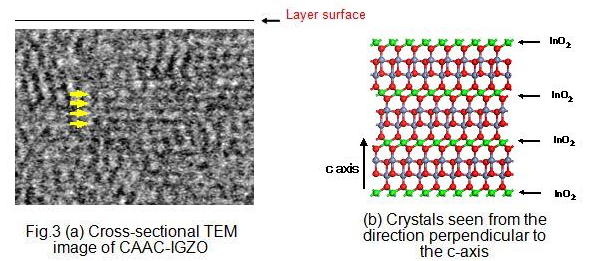
\includegraphics[width=1\linewidth]{IMMAGINI/immagine_cristalizzazione_CAAS}
			\caption{Crystals}
			\label{fig:immaginecristalizzazionecaas}
		\end{figure}
	\end{frame}
	\begin{frame}
		\frametitle{Display AMOLED pieghevoli: Trasferimento tecnologico}
		\begin{itemize}
			\item Il processo di trasferimento tecnologico richiede un array di transistor field-effect (FET) formati da un substrato di vetro che è separato da un livello inorganico
			\pause
			\item  Permette di ottenere \textbf{alte performance} e \textbf{alta affidabilità}	
		\end{itemize}
	\end{frame}
	\begin{frame}
		\frametitle{Trasferimento tecnologico: processo produttivo}
		\begin{figure}
			\centering
			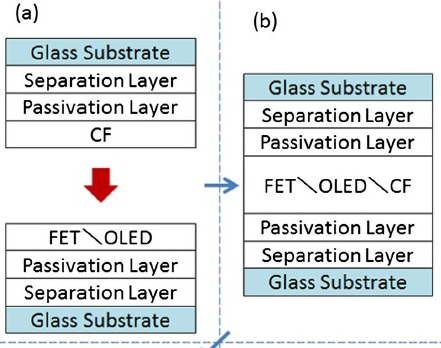
\includegraphics[width=0.7\linewidth]{FISICA/tabella_formazione1}
			\caption{Processo produttivo}
			\label{fig:tabellaformazione1}
		\end{figure}
	\end{frame}
	\begin{frame}
		\frametitle{Trasferimento tecnologico: processo produttivo}
		\begin{figure}
			\centering
			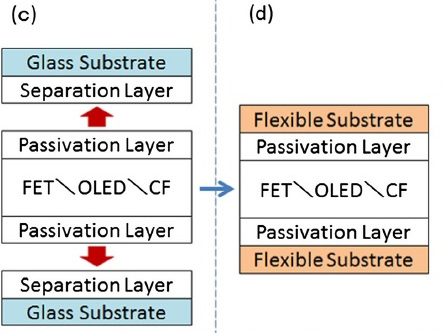
\includegraphics[width=0.7\linewidth]{FISICA/tabella_formazione2}
			\caption{Processo produttivo}
			\label{fig:tabellaformazione2}
		\end{figure}
	\end{frame}
	\begin{frame}
		\frametitle{Test di piegatura schermo}
		\begin{figure}
			\centering
			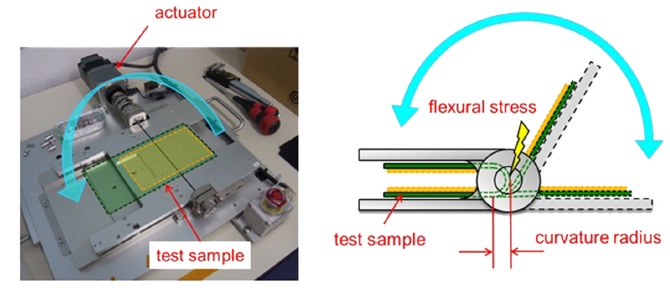
\includegraphics[width=1\linewidth]{FISICA/test2}
			\caption{Test di piegatura}
			\label{fig:test2}
		\end{figure}
	\end{frame}
	\begin{frame}
		\frametitle{Test su pannello flessibile ad alte temperature e alte umidità}
		\begin{figure}
			\centering
			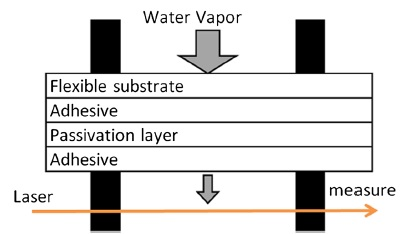
\includegraphics[width=1\linewidth]{FISICA/test_temp}
			\caption{Test di temperatura e umidità}
			\label{fig:testtemp}
		\end{figure}
	\end{frame}
	\begin{frame}
		\frametitle{Test su pannello flessibile ad alte temperature e alte umidità}
		\begin{itemize}
			\item Dopo ben 500 ore non è stato possibile osservare alcun punto nero dei pixel e nemmeno restringimento dei pixel
			\pause
			\item Si può concludere che il livello passivo ha una buona affidabilità e qualità costruttiva
		\end{itemize}
	\end{frame}
	\begin{frame}
		\frametitle{Sfida tecnologica per implementare schermi AMOLED di grandi dimensioni}
		Si va ad analizzare alcune tecnologie come:
		\begin{itemize}
			\item L’ossido di TFTs combinato con i vantaggi
			del LTPS e a-Si TFTs. Questi portano dei vantaggi su schermi molto grandi
			\pause
			\item Comparazione tra ossido dei TFTs con l'uso dell'ELA LTPS e l'uso di IGZO amorfo
		\end{itemize}
	\end{frame}
	\begin{frame}
		\frametitle{3 punti fondamentali per gli schermi}
		\begin{itemize}
			\item \textbf{Fabbricazione e performance dei TFT}
			\pause
			\item \textbf{Il design degli OLED} 
			\pause
			\item \textbf{L'incapsulamento degli schermi}
		\end{itemize}
	\end{frame}
	\begin{frame}
		\frametitle{Sfida tecnologica: introduzione delle tecnologie}
		\begin{itemize}
			\item Un primo approccio per la creazione di un pannello posteriore dell'OLED è stato creare una metodologia, per la creazione di TFT, che si basa su ELA e LTPS
			\pause
			\item Queste tecniche sono valide sia per la loro \textbf{\textcolor{green}{mobilità}} che \textbf{\textcolor{green}{stabilità}} 
		\end{itemize}
	\end{frame}
	\begin{frame}
		\frametitle{Sfida tecnologica: introduzione delle tecnologie}
		\begin{itemize}
			\item Ma come tutte le tecniche, anche queste hanno delle \textbf{limitazioni} derivanti dai raggi laser che vengono impiegati per lo sviluppo di questa tecnica (ELA)
		\end{itemize}
	\end{frame}
	\begin{frame}
		\frametitle{Sfida tecnologica: introduzione delle tecnologie}
		\begin{itemize}
			\item Seconda tecnologia implementata è la \textbf{fine metal shadow mask} (FMM), cioè una maschera che viene posta tra i diversi strati per introdurre i colori primari all'interno dello schermo OLED
			\pause
			\item Presenta delle limitazioni aumentando la dimensione dell'area da ricoprire
		\end{itemize}
	\end{frame}
	\begin{frame}
		\frametitle{Sfida tecnologica: introduzione delle tecnologie}
		\begin{itemize}
			\item Ci sono alcune soluzione valide per la sostituzione della FMM, quali per esempio: Laser-based patterning methods, radiation-induced sublimation transfer (RIST), laser-induced pattern-wise sublimation (LIPS) and laser-induced thermal transfer (LITI)
		\end{itemize}
	\end{frame}
	\begin{frame}
		\frametitle{Stato di corrente e problemi sulla tecnologia di cristallizzazione}
		\begin{itemize}
			\item Ci sono 4 principali problemi che riguardano il pannello posteriore di uno schermo OLED
		\end{itemize}
	\end{frame}
	\begin{frame}
		\frametitle{Stato di corrente e problemi sulla tecnologia di cristallizzazione}
		\begin{itemize}
			\item Riduzione del numero di 'photo-mask'
			\pause
			\item Miglioramento della luminosità non uniforme
			\pause
			\item IR drop prevention (introdurre un elettrodo di supporto per prevenire una rottura dovuta ad un salto di tensione)
			\pause
			\item Affidabilità del device
		\end{itemize}
	\end{frame}
	\begin{frame}
		\frametitle{Stato di corrente e problemi sulla tecnologia di cristallizzazione}
		\begin{itemize}
			\item La creazione del LCD attraverso a-Si (Silicio Amorfo) permette di avere costi bassi in merito alla fabbricazione, ma non permette di ottenere delle prestazioni altrettanto buone
		\end{itemize}
	\end{frame}
	\begin{frame}
		\frametitle{Stato di corrente e problemi sulla tecnologia di cristallizzazione}
		\begin{itemize}
			\item Per ottenere prestazioni migliori di solito, al giorno d'oggi, viene utilizzato il Si LTPS, ovvero, silicio policristallino a basse temperature
			\pause
			\item Fornisce così una migliore \textbf{mobilità} e \textbf{stabilità}
			\pause
			\item \textbf{\textcolor{green}{Processo chiave:}} trasformare a-Si in Si policristallino
		\end{itemize}
	\end{frame}
	\begin{frame}
		\frametitle{Cristallizzazione senza l'ausilio di laser}
		\begin{itemize}
			\item Senza laser: il processo richiede una temperatura che stia sui 600 \degree C, con una cottura che dura all'incirca una decina d'ore
			\pause
			\item Questa soluzione se non fatta in maniera precisa porta ad avere delle crepe nella fase di cristallizzazione
		\end{itemize}
	\end{frame}
	\begin{frame}
		\frametitle{Cristallizzazione ELA}
			\begin{figure}
				\centering
				\includegraphics[width=1\linewidth]{"FISICA/ELA cristallizzazione"}
				\caption{ELA}
				\label{fig:ela-cristallizzazione}
			\end{figure}
	\end{frame}
	\begin{frame}
		\frametitle{ELA (excimer laser annealing) vantaggi}
		\begin{itemize}
			\item \textbf{\textcolor{green}{Eccellente cristallizzazione, veloce cristallizzazione e un'alta mobilità}}
		\end{itemize}
	\end{frame}
	\begin{frame}
		\frametitle{ELA (excimer laser annealing) svantaggi}
		\begin{itemize}
			\item \textbf{\textcolor{red}{Alto costo di mantenimento e fabbricazione, lunghezza e instabilità del raggio laser su piani di grandi dimensioni}}
		\end{itemize}
	\end{frame}
	\begin{frame}
		\frametitle{Alternativa di ELA}
		\begin{itemize}
			\item Si uniscono i vantaggi derivanti da a-Si e LTPS
		\end{itemize}
	\end{frame}
	\begin{frame}
		\frametitle{Processo produttivo a-Si e LTPS}
		\begin{itemize}
			\item Molto simile al processo che viene fatto attraverso a-Si
			\pause
			\item In aggiunta al processo produttivo "standard" viene inserito l'ossido di TFT in una camera di temperatura
		\end{itemize}
	\end{frame}
	\begin{frame}
		\frametitle{Processo produttivo a-Si e LTPS}
		\begin{figure}
			\centering
			\includegraphics[width=1\linewidth]{"FISICA/produzione LTPS + a-Si"}
			\caption{a-Si + LTPS}
			\label{fig:produzione-ltps--a-si}
		\end{figure}
	\end{frame}
	\begin{frame}
		\frametitle{Tecnologia Ossido TFT}
		\begin{figure}
			\centering
			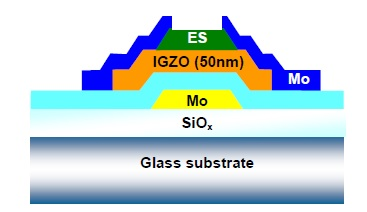
\includegraphics[width=1\linewidth]{FISICA/ossidoTFT}
			\caption{Ossido TFT}
			\label{fig:ossidotft}
		\end{figure}
	\end{frame}
	\begin{frame}
		\frametitle{Tecnologia Ossido TFT}
		\begin{figure}
			\centering
			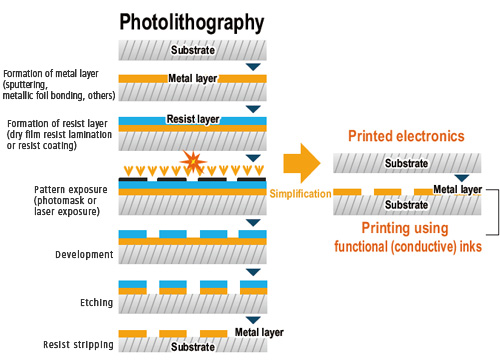
\includegraphics[width=0.9\linewidth]{IMMAGINI/photolitography}
			\caption{Photolithography}
			\label{fig:photolitography}
		\end{figure}
	\end{frame}	
	\begin{frame}
		\frametitle{Implementare schermi AMOLED di grandi dimensioni: conclusioni}
		\begin{itemize}
			\item In definitiva si è sviluppato un display WXGA AMOLED full-color da 12.1 inch
			\pause
			\item Per la realizzazione del display si è utlizzato \textbf{a-IGZO}
			\pause
			\item Alla fine il processo, attraverso il quale si è realizzato il pannello posteriore del display, può essere facilmente esteso in una produzione di grandi schermi, potendo utilizzare tecniche, quali sputtering per la creazione dei canali 
		\end{itemize}
	\end{frame}
\end{document}